\documentclass[runningheads,a4paper]{article}

\usepackage[utf8]{inputenc}
 
\setcounter{tocdepth}{3}

\usepackage[english]{babel} 
\usepackage{graphicx}
\usepackage{grffile}
\usepackage{float}
\usepackage{multicol}
\usepackage{url}
 
\usepackage{titling}
\usepackage[hidelinks]{hyperref}
\setcounter{secnumdepth}{5}
%Margins
\usepackage[
margin=2cm,
includefoot
]{geometry}


\graphicspath{{img/}}

%Headers and Footers
\usepackage{fancyhdr}
\pagestyle{fancy}
\fancyhead{}
\fancyfoot{}
\fancyfoot[R]{\thepage}
\renewcommand{\headrulewidth}{0pt}
\renewcommand{\footrulewidth}{0pt}
 \setlength\parindent{24pt}
\begin{document}

	%Title Page
	\begin{titlepage}
		\begin{center}
			
\includegraphics[width=10cm]{UP.jpg}  \\
			[1cm]
			\line(1,0){300} \\
			[0.3cm]
			\textsc{\Large
				NavUP\\
				Software Requirements Specification\\
			\hfill \break 24 February 2017
				%University of Pretoria
			}\\
			[0.1cm]
			\line(1,0){300} \\
			[0.7cm]
			\textsc{\Large
				Team Indigo
			} \\
			
			
			
		\end{center}
		
		\begin{center}
			\begin{multicols}{2}
				\textsc{\large\\
				Andries du Plooy\\ 
					15226183\\ 
				}
				
				\textsc{\large\\
				Vignesh Iyer\\
					 15031625\\ 
				}
				
				\textsc{\large\\
		        Mfana Masimula\\
				 	12077713\\ 
				}
				
				\columnbreak
				
				\textsc{\large\\
					 Avinash Singh\\
					14043778\\
				}
				
				\textsc{\large\\
					Nicaedin Suklal\\
					15207812\\
				}
				
			\end{multicols}
			
			
			\textsc{	\\ \href{https://github.com/AndriesJacobus/SE-Indigo}{GitHub}
				\url{https://github.com/AndriesJacobus/SE-Indigo.git}}
			
		\end{center}
	\end{titlepage}
%\maketitle

\begingroup

\tableofcontents
\addcontentsline{toc}{section}{Table Of Contents}
\endgroup
\newpage


\section{Introduction}

\subsection{Purpose}
The purpose of this Software Requirements Specification Document is to lay out the findings of a standardised requirements elicitation for the proposed application. In doing this, both the capabilities that the application is expected to deliver together, with the constraints on the solution space are described.\newline \newline The document will take into account requirements, as set out by both the developers and the prospective users, in order to lay a foundation for the up-coming phases of the Software Development Cycle. The various sections each provide details on specific types of requirements of the application.\newline \newline The intended audience include developers/peers(Team Indigo and other COS 301 teams), domain experts(COS 301 Lectures and the University of Pretoria Management), customers/end-users(students, staff and visitors at the University of Pretoria) who will perform a technical, expert  and customer review of this document respectively.
 
\subsection{Scope}
The name of the proposed software application is NavUP (NavigationUP). NavUP is intended to be an information service application that is to provide navigational information to visitors, employees and students of the University of Pretoria. This includes usual navigational functions (mapping and routing of campus), surveillance, user based information delivery and event calenders. NavUP will not extend its functionalities outside the Hatfield Campus and the University of Pretoria will not take any responsibility for any injury, damage or whatsoever that may be a result of the application. The application is used at your own risk.\newline \newline The objectives of the product include making the University of Pretoria feel more "like home" to all stakeholders alike. The application aims to facilitate a wide range of users who have had difficulties in the past with regard travelling within the premises. Ease of travel, accessibility of the various facilities, time optimisations, event/day-to-day coordination's, alleviating pedestrian traffic congestion problems, description of activities etc. are the joint objectives of the project.\newline \newline The goal is to integrate existing applications within the university like the Wi-Fi hotspots, IT-Services, Official University Website, Social Media and more.  Another goal is for the application to make use of human resources for its development and usage i.e. expertise from the COS 301, Honours groups of students and lectures to satisfy the former and make use of crowd-sourcing principles (using smart devices) to serve the latter. \newline \newline The benefits include smoothness of the day-to-day operations at the University which leads to greater productivity and efficiency among students and staff alike. It allows the university to increase its brand value in terms of the facilities it provides to keep external stakeholders pleased. National and Global Rankings of the university are bound to rise and consequently attract a larger group of people in the long run.

\subsection{Definitions, Acronyms, and Abbreviations}
\paragraph{\textbf{Acronyms}}
\begin{enumerate}
	\item Wi-Fi - Wireless Fidelity 
	\item SHA - Simple Hashing Algorithm
	\item UI - User Interface
	\item UX - User Experience
	\item GPS - Global Positioning System
	\item AP - Access points
	\item SRS - Software Requirements Specification
	\item IEEE - Institute of Electrical and Electronic Engineers 
	\item UP - University of Pretoria
	\item IOS - iPhone Operating System 
	\item IT - Information Technology
	\item NavUP - Navigation University of Pretoria
	\item 2D - Two Dimensional
	\item 3D - Three Dimensional
	\item SRC - Student Representative Council
	\item RUTM - Requirement Use Case Tracebility Matrix
\end{enumerate}

\paragraph{\textbf{Abbreviations}}
\begin{enumerate}
	\item STD - Standard
	\item App - Application
	\item Info - Information
\end{enumerate}

\subsection{References}
Kung, D.C. (2013) Object-oriented software engineering: An agile unified methodology. New York: McGraw Hill Higher Education.

\subsection{Overview}
The rest of this document will be solely focussed on elaborating on the requirements of the NavUP application. It is structured according to the IEEE STD 830-1998 standard. An overall description of the product will be followed by a specific detailed requirements description. Each item in both the sections represent the ideas as generated during compilation and there is possibilities of change during the implementation of the application.

\section{Overall Description}

\subsection{Product Perspective}

\subsubsection{System Interfaces}
\paragraph{...}
\subsubsection{User Interfaces}
\paragraph{...}
\subsubsection{Hardware Interfaces}
\paragraph{...}
\subsubsection{Software Interfaces}
\paragraph{...}
\subsubsection{Communication Interfaces}
\paragraph{...}
\subsubsection{Memory}
\paragraph{...}
\subsubsection{Operations}
\paragraph{...}
\subsubsection{Site Adaptation Requirements}
\paragraph{...}

\subsection{Product Functions}
\paragraph{...}
\subsection{User Characteristics}
\paragraph{...}
\subsection{Constraints}
\paragraph{...}

 
\subsection{Assumptions and Dependencies}
%\let\labelitemi\labelitemii
The factors that affect the requirements are:
\begin{itemize}
	 
		\item Lack of connectivity -  Wi-Fi isn't available everywhere on campus (e.g. I.T building). Thus, assuming that Wi-Fi on campus will essentially be available everywhere in due time, and/or mobile network fall-back is assumed.
		
		\item Mobile devices - It is assumed that a user will have a mobile device that can run the application; it must specifically be able to run the newer versions of Android, IOS and Windows Mobile. We assumed that the mobile device was powerful enough to draw maps and emulate navigation.
		\item Server - The application depends on running on a remote server where the mobile application can authenticate and gain essential information to navigation.
		
		\item Hotspots - We assumed that the Wi-Fi Hotspots on campus will be forever lasting and we depend on this application to triangulate and refine navigation on the application.
	 
\end{itemize}
 


\section{Specific Requirements}

\subsection{External Interface Requirements}
\paragraph{...}
\subsection{Functional Requirements}

\subsubsection{User Login}
\textbf{Description:}  The application will provide the ability for users to login. Students and staff have their UP Portal accounts linked to the NavUP system database will input their respective usernames and passwords. Guests/Visitors will click "Guest Log-in" instead of credentials. The system database will verify the credentials (processing) and output returns to the current screen on "error" or the application home page on "success".\\\\
\noindent
\textbf{Prioritisation:} Important\\
  
  
\textbf{Pre-conditions}
\begin{itemize}
 	\item A user must have a connection to the server.
  	\item A user must be registered with the University (staff/student), or be a visitor within the Hatfield premises.
  	\item The user must enter the correct information in order for the authentication to be successful.
\end{itemize}
  
\textbf{Post-conditions}
\begin{itemize}
  	\item The user has specific access to the server on which all data is stored, i.e add/edit locations, meta-data and search locations, buildings, rooms etc.
  	\item The user is able to use all the user functionality provided by the system. 
  	\item The user may log out of the system when they wish to.
\end{itemize}
  
\begin{figure}[H]
   	\centering
   	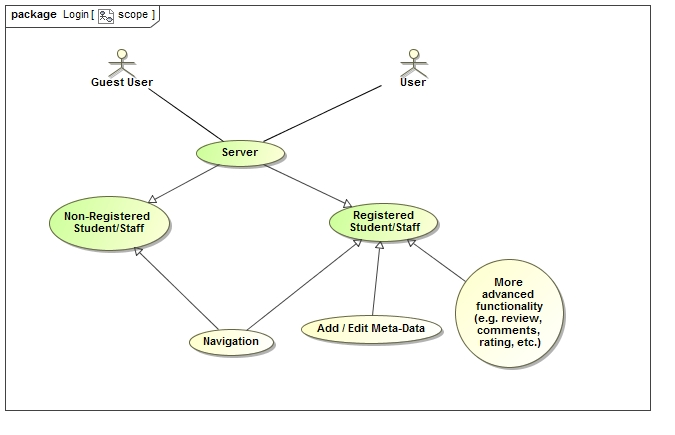
\includegraphics[width=0.7\textwidth]{LoginActorSystem.jpg}
   	\caption{Actor System: User Login}
\end{figure}
  

\noindent \underline{Interactive graphical map of the University of Pretoria's Hatfield Campus - }\\
\noindent \underline{both indoor and outdoor structures will be mapped.}\\
\noindent \underline{Functions associated with this are described below:}

\subsubsection{Map Scroll}

\textbf{Description:}  The application will accept user input (a pointing device or touch screen) which can be processed to produce output of scrolling the map around and within its boundaries and viewing the various symbolic representations of the University premises.\\\\
\noindent
\textbf{Prioritisation:} Important\\
  
  
\textbf{Pre-conditions}
\begin{itemize}
 	\item A user must have a working touch screen sensitivity or a pointing device.
\end{itemize}
  
\textbf{Post-conditions}
\begin{itemize}
%  	\item NONE
	\item The map will be moved to the position where the user scrolled. 
\end{itemize}

\subsubsection{Map Zoom}

\textbf{Description:}  The application will accept user input of pinching the screen (Two fingers on the edges of a map are spread apart to enlarge the images or brought together to make the map smaller). The processing will be of the positions on the screen of the fingers and output will be a screen image which has changed size.\\\\
\noindent
\textbf{Prioritisation:} Important\\
  
  
\textbf{Pre-conditions}
\begin{itemize}
 	\item A user must have a working touch screen sensitivity or a pointing device.
\end{itemize}
  
\textbf{Post-conditions}
\begin{itemize}
%  	\item NONE
	\item The map will zoomed in/out the amount the user pinched on the screen. 
\end{itemize}

\subsubsection{Map Query}

\textbf{Description:}  The application will provide a map query feature by means of a search bar input. Input can range from names of buildings, lecture halls, faculties, schools, departments, restaurants and coffee shops, shops, laboratories, libraries, study centres, offices, toilets,  parking facilities, gate numbers, streets and student organisations and day houses. NavUP will auto-scroll the map to the location as output if identification is successful. Otherwise, it will provide you with “Did you mean to say …” options or “Location could not be found” output (error output).\\\\
\noindent
\textbf{Prioritisation:} Important\\
  
  
\textbf{Pre-conditions}
\begin{itemize}
 	\item The user must be connected to the server for the input to be processed.
	\item The input must be keywords which are short and precise for successful identification.
\end{itemize}
  
\textbf{Post-conditions}
\begin{itemize}
  	\item The user has the ability to either choose from a list of options or the system state moves to representing the user's search.
\end{itemize}

\subsubsection{Save Map Location}

\textbf{Description:}  The application will give users the privileges of saving locations (database save) by an input of pinning - pinpoint locations manually by clicking (input) the marker icon and placing it directly onto the map. Locations of modules which the user has registered for will automatically be pinned. The output will be that of a red pin on the location which was scrolled over.\\\\
\noindent
\textbf{Prioritisation:} Important\\
  
  
\textbf{Pre-conditions}
\begin{itemize}
 	\item The user must be connected to the server during the pinning operation.
	\item The user should be a student or staff member to exercise this feature - visitors have no active account for a database save.
	\item Registration of modules should have taken place at least 24 hours before the application can auto-pin the modules.
\end{itemize}
  
\textbf{Post-conditions}
\begin{itemize}
  	\item The user will have a record corresponding to his student/staff number for this pin operation in the database.
\end{itemize}

\subsubsection{See Location Information}

\textbf{Description:}  NavUP will allow more prominent locations to be clicked (input) after which a pop-up (output) will appear with any one or both of the following: a general description of the location and information about activities and events set to take place there.\\\\
\noindent
\textbf{Prioritisation:} Important\\
  
  
\textbf{Pre-conditions}
\begin{itemize}
 	\item The feature is limited to important locations (academic hubs, cultural sites).
	\item The user must be connected to the server for information to be retrieved.
\end{itemize}
  
\textbf{Post-conditions}
\begin{itemize}
  	\item The information location will be provided to the user.
\end{itemize}

\subsubsection{Change Map Type}

\textbf{Description:}  NavUP will provide the users with a toggle button (input) to switch between normal map view as described above and a traffic congestion map (hot-zone map) – this map is coloured according to the relative traffic flow in various parts of campus (in shades of red) taking into account the number of Wi-Fi users in and around hotspots in the particular area.\\\\
\noindent
\textbf{Prioritisation:} Important\\
  
  
\textbf{Pre-conditions}
\begin{itemize}
 	\item The Wi-Fi must be up and running for the traffic congestion map to be displayed.
	\item The user must be connected to the server for information to be retrieved.
\end{itemize}
  
\textbf{Post-conditions}
\begin{itemize}
  	\item Map state changes depending on the type of map being viewed.
\end{itemize}


%\let\labelitemi\labelitemii

\noindent \\ \underline{A Directional Search is feature will be provided by the application and will contain the following functionality:}


\subsubsection{Highlight Directions on Map}

\textbf{Description:}  Clicking/pressing (input) on the direction symbol will open up two different fields: a starting point and destination field. Both fields accept the same input and are constrained by the same error-checking as was for the map query function.
The route from the starting point to the end point (both encircled) will be highlighted on the map (output) with a bold colour and the section of the map will come into focus as soon as the search button is clicked/pressed (input).\\\\
\noindent
\textbf{Prioritisation:} Important\\
  
  
\textbf{Pre-conditions}
\begin{itemize}
	\item The user must be connected to the server for information to be retrieved.
\end{itemize}
  
\textbf{Post-conditions}
\begin{itemize}
  	\item Map state changes depending on the type of map being viewed.
\end{itemize}

\subsubsection{Turn-By-Turn Navigation}

\textbf{Description:}  The application will map (processing) the user (represented by his electronic device) with regard to his proximity to a Wireless Router (all users making use of the Hatfield Wi-Fi are mapped in this way). NavUP will provide the user with turn-by-turn navigation directions towards their destination as they move with their device (input) and the device connects to various Wi-Fi routers (processing) – both in terms of a moving Stick Man and automated voice instructions (output).\\\\
\noindent
\textbf{Prioritisation:} Important\\
  
  
\textbf{Pre-conditions}
\begin{itemize}
	\item The user must be connected to the server for information to be retrieved.
	\item The user must have in-built speakers or earphones to be able to hear the instructions.
	\item All Wi-Fi hotspots must be working for triangulation to take place.
\end{itemize}
  
\textbf{Post-conditions}
\begin{itemize}
  	\item The user will receive turn-by-turn navigation provided by the map and voice instructions.
\end{itemize}

\subsubsection{Automatic Re-Route}

\textbf{Description:}  The application will make re-routing possible if the user does not move in the initial prescribed route (processing new directions). Input is that of moving with the device in the wrong direction. Distance costs of the various routes will be displayed by the software (output) and the user has to make an initial choice on which route they would like to follow (input).\\\\
\noindent
\textbf{Prioritisation:} Important\\
  
  
\textbf{Pre-conditions}
\begin{itemize}
	\item The user must be connected to the server for information to be retrieved.
\end{itemize}
  
\textbf{Post-conditions}
\begin{itemize}
  	\item The route will be re-calculated and displayed so that navigation can be relevant and accurate.
\end{itemize}

\subsubsection{Route Without Traffic}

\textbf{Description:}  NavUP provides the integration of traffic congestion information with routing (a check-box input is provided to enable this feature before the routing is processed) to allow users to choose routes where there is a less gathering of people (in terms of number of Wi-Fi connections alternative options are suggested).\\\\
\noindent
\textbf{Prioritisation:} Important\\
  
  
\textbf{Pre-conditions}
\begin{itemize}
	\item The user must be connected to the server for information to be retrieved.
\end{itemize}
  
\textbf{Post-conditions}
\begin{itemize}
  	\item The best possible route without traffic will be presented to the user.
\end{itemize}

\subsubsection{Monitor Fitness}

\textbf{Description:} The application also integrates with the UP Fitness Trail route – directional information together with monitoring an embedded stopwatch (runs on the foreground as output) is provided for this feature. Users will be able to save their progress to their accounts (database processing on click of save button input).\\\\
\noindent
\textbf{Prioritisation:} Important\\
  
  
\textbf{Pre-conditions}
\begin{itemize}
	\item The user must be connected to the server for information to be retrieved.
	\item This feature is only available to UP staff and students.
\end{itemize}
  
\textbf{Post-conditions}
\begin{itemize}
  	\item The user should have completed the fitness trial.
	\item The stopwatch returns to initial state.
\end{itemize}

\noindent \\ \underline{NavUP will is based on a “push technology” model and as a result provides the following functionality:}

\subsubsection{View Calendar}

\textbf{Description:} The application will have a tab (click on the tab as input) which displays (output) a calendar of events (special guest lectures, music and dance festivals, religious gatherings, graduation ceremonies, meetings, information sessions etc.).\\\\
\noindent
\textbf{Prioritisation:} Medium Priority\\
  
  
\textbf{Pre-conditions}
\begin{itemize}
	\item The University of Pretoria should integrate their calendar with that of NavUP.
	\item All events must be communicated to the system administrator for them to be displayed.
\end{itemize}
  
\textbf{Post-conditions}
\begin{itemize}
  	\item The calendar with the events will be displayed to the user.
\end{itemize}

\subsubsection{Set Reminder}

\textbf{Description:} The user can interact with the calendar by clicking on specific events or dates to set remainders ("SAVE THIS DATE" check-box). The output is of the date being highlighted on calendar view.\\\\
\noindent
\textbf{Prioritisation:} Medium Priority\\
  
  
\textbf{Pre-conditions}
\begin{itemize}
	\item The user must be a staff member or a student of UP.
\end{itemize}
  
\textbf{Post-conditions}
\begin{itemize}
  	\item The reminder will be set on the users device.
\end{itemize}

\subsubsection{Push Notifications}

\textbf{Description:} When connected to the Wi-Fi, the user can get a push notification slide down from the top of the screen when the event date has occurred (processing is always taking place in the background in order to check which user events are active on a specific date).\\\\
\noindent
\textbf{Prioritisation:} Medium Priority\\
  
  
\textbf{Pre-conditions}
\begin{itemize}
	\item The user must be a staff member or a student of UP.
	\item Push Notifications must be enabled.
\end{itemize}
  
\textbf{Post-conditions}
\begin{itemize}
  	\item The user has the ability to act on this notification i.e. clear it or ask for directions to the venue mentioned on it.
\end{itemize}

\subsubsection{Show event route}

\textbf{Description:} The application allows the user to then click on “Show event route”, which provides the various mapping and routing options described above as output.\\\\
\noindent
\textbf{Prioritisation:} Medium Priority\\
  
  
\textbf{Pre-conditions}
\begin{itemize}
	\item The user must have at least one event with a location available to navigate too.
\end{itemize}
  
\textbf{Post-conditions}
\begin{itemize}
  	\item The selected events route will be set as the users navigation destination.
\end{itemize}

\subsubsection{Add An Event}

\textbf{Description:} The application allows an event to be added. Input includes name of event, date, venue, purpose, targeted audience, dress code, time and event capacity. The event will be added to the events database table (processing). Output will be visible in "View Calendar".\\\\
\noindent
\textbf{Prioritisation:} Medium Priority\\
  
  
\textbf{Pre-conditions}
\begin{itemize}
	\item Only staff members, SRC members and management can add events.
\end{itemize}
  
\textbf{Post-conditions}
\begin{itemize}
  	\item The event will be successfully added to the system.
\end{itemize}

\subsubsection{Identified Use Cases}
\textbf{Requirements are rephrased as business processes:}
\begin{itemize}
	\item UC1 - Log in User
	\item UC2 - Scroll Map
	\item UC3 - Zoom Map
	\item UC4 - Query Map
	\item UC5 - Save Map Location
	\item UC6 - View Map Location Information
	\item UC7 - Switch Map
	\item UC8 - View Directions
	\item UC9 - Provide Turn-by-Turn Directions
	\item UC10 - View Traffic-less Directions
	\item UC11 - Provide Traffic-less Directions
	\item UC12 - Monitor Fitness
	\item UC13 - View Calendar
	\item UC14 - Set Reminder
	\item UC15 - Enable Push-Notifications
	\item UC16 - Add Event 
\end{itemize}


\subsubsection{Requirement Use Case Tracebility Matrix}

\begin{table}[]
\centering
\caption{Traceability Matrix - Too large to fit - Part 1}
\label{my-label}
\begin{tabular}{|l|l|l|l|l|l|l|l|l|l|}
\hline
Requirements & Priority & UC1 & UC2 & UC3 & UC4 & UC5 & UC6 & UC7 & UC8 \\ \hline
3.2.1 & 1 & x &  &  &  &  &  &  &  \\ \hline
3.2.2 & 1 &  & x &  &  &  &  &  &  \\ \hline
3.2.3 & 1 &  &  & x &  &  &  &  &  \\ \hline
3.2.4 & 1 &  &  &  & x &  &  &  &  \\ \hline
3.2.5 & 2 &  &  &  &  & x &  &  &  \\ \hline
3.2.6 & 2 &  &  &  &  &  & x &  &  \\ \hline
3.2.7 & 2 &  &  &  &  &  &  & x &  \\ \hline
3.2.8 & 1 &  &  &  &  &  &  &  & x \\ \hline
3.2.9 & 1 &  &  &  &  &  &  &  &  \\ \hline
3.2.10 & 2 &  &  &  &  &  &  &  &  \\ \hline
3.2.11 & 2 &  &  &  &  &  &  &  &  \\ \hline
3.2.12 & 4 &  &  &  &  &  &  &  &  \\ \hline
3.2.13 & 3 &  &  &  &  &  &  &  &  \\ \hline
3.2.14 & 4 &  &  &  &  &  &  &  &  \\ \hline
3.2.15 & 3 &  &  &  &  &  &  &  &  \\ \hline
3.2.16 & 3 &  &  &  &  &  &  &  & x \\ \hline
3.2.17 & 4 &  &  &  &  &  &  &  &  \\ \hline
\multicolumn{2}{|l|}{UC Priority} & 1 & 1 & 1 & 1 & 2 & 2 & 2 & 1 \\ \hline
\end{tabular}
\end{table}

\begin{table}[]
\centering
\caption{Traceability Matrix - Continuation - Part 2}
\label{my-label}
\begin{tabular}{|l|l|l|l|l|l|l|l|l|l|}
\hline
Requirements      & Priority      & UC9 & UC10 & UC11 & UC12 & UC13 & UC14 & UC15 & UC16 \\ \hline
3.2.1             & 1             &     &      &      &      &      &      &      &      \\ \hline
3.2.2             & 1             &     &      &      &      &      &      &      &      \\ \hline
3.2.3             & 1             &     &      &      &      &      &      &      &      \\ \hline
3.2.4             & 1             &     &      &      &      &      &      &      &      \\ \hline
3.2.5             & 2             &     &      &      &      &      &      &      &      \\ \hline
3.2.6             & 2             &     &      &      &      &      &      &      &      \\ \hline
3.2.7             & 2             &     &      &      &      &      &      &      &      \\ \hline
3.2.8             & 1             &     &      &      &      &      &      &      &      \\ \hline
3.2.9             & 1             & x   &      &      &      &      &      &      &      \\ \hline
3.2.10            & 2             & x   &      & x    &      &      &      &      &      \\ \hline
3.2.11            & 2             &     & x    & x    &      &      &      &      &      \\ \hline
3.2.12            & 4             &     &      &      & x    &      &      &      &      \\ \hline
3.2.13            & 3             &     &      &      &      & x    &      &      &      \\ \hline
3.2.14            & 4             &     &      &      &      &      & x    &      &      \\ \hline
3.2.15            & 3             &     &      &      &      &      &      & x    &      \\ \hline
3.2.16            & 3             & x   & x    & x    &      &      &      &      &      \\ \hline
3.2.17            & 4             &     &      &      &      &      &      &      & x    \\ \hline
\multicolumn{2}{|l|}{UC Priority} & 1   & 1    & 2    & 3    & 3    & 4    & 3    & 4    \\ \hline
\end{tabular}
\end{table}


\pagebreak

\subsubsection{Use Cases Partitioned Among Systems}
\begin{figure}[H]
   	\centering
   	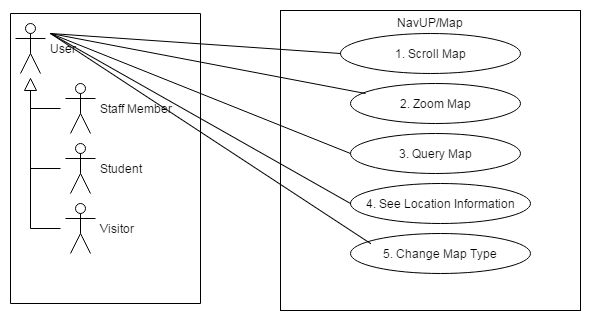
\includegraphics[width=0.7\textwidth]{NavUP-Map-Subsystem.jpg}
   	\caption{Map Sub-system}
\end{figure}

\subsection{Performance Requirements}

%\let\labelitemi\labelitemii

\noindent \\ Real-Time Processing

\begin{itemize}
\item Map Search Algorithm\\The search algorithm should be efficient – keywords specified by the user needs to be hashed to find the location on the map. A time-complexity of Big-O(1) is achieved. A hash-table with possible keywords need to be matched to locations on the map.

\item Directional Search Algorithm\\The routes determined must be least cost routes in terms of distance and in terms of traffic rates – Djikstra’s algorithm.

\item User Location Determination\\The coordination of the Wi-Fi hotspots in determining user location should be to a precision that allows an error-rate of no more than 7 metres.

\item Re-Routing\\A time-elapse of no more than 5 seconds is allowed when the system has to re-calculate the routes.

\item Capacity\\The system must have the ability to handle requests from a minimum of 1000 users. Around 10000 requests can be made to the user on average in a day.

\item Interactiveness and Response Time\\The system must be interactive and the delays involved must be less. The opening of tabs, pop-ups, dialog boxes, switching between traffic and terrestrial maps, scrolling up and across the scene and zooming in and out of the map should all have quick response time - these functions need to be initiated within two seconds submitting them to the system in the form of click/scroll input.

\item System Dependability\\If the system loses the connection to the Wi-Fi or gets some gibberish input to which it transitions to an unstable state, the user should be informed rather then there being stagnant instances of time.

\end{itemize}

\subsection{Design Constraints}
\paragraph{...}

 
\subsection{Software System Attributes}
\subsubsection{Quality Requirements }
The following section will focus on the quality requirements of the overall system and mobile application at its highest level of granularity. All the requirements defined, are for all components of the system.

\paragraph{\textbf{Reliability}\\}
The system and application should be reliable in the fact that the user should be able to reach his/her destination and that the information provided by the system and application is accurate and authentic. The system should always be on-line and provide the expected functionality without errors or discrepancies. The system should also provide additional information aiding the reliability by giving a short description or history of the building or venue to make it more reliable and accurate. 

\paragraph{\textbf{Security}\\}
Although security is not a key feature, the system should protect any personal information by hashing passwords with a secure hashing algorithm such as SHA-256 or SHA-512 and not leak any information from the system or application. The application should have access to the users Wi-Fi connections as well as cellular fall-back for enhanced navigation and even GPS. The system or application should not store any Wi-Fi information from the device or pull user-names and passwords from the users device and leak it.
We will achieve security by making use of 3 methods, namely: prevention, detection, and recovery. We will ensure that we have put means in
place through which we may be able to detect any threats to the system,
for example, validating any information that is required to be sent to the
server. Preventing threats to the system can be enforced through limiting the access channels, making use of authentication, not allowing any
external sources to be accessed through the system, etc. Recovery will be
achieved through cancelling requests and maintaining a working back up
state to roll back changes.  

\paragraph{\textbf{Availability} \\}
 The system should be available at all times and the mobile application available to most recent types of user devices and operating systems on these devices. The system should always be on-line except if there is no Wi-Fi connectivity.

\paragraph{\textbf{Flexibility} \\}
 An important element of the system is its flexibility. 
 Each component of the system should be decoupled from every other component, thus allowing you to change certain components without affecting anything else. 
 For example, it should be easy to add a new Lecture Venue to the system with little or no code modifications. 
 The main focus of the software is to allow the user to easily navigate to his/her destination with minimal effort.
 In spite of this, the navigation route should be flexible in the sense there could be many different routes that the user can take and the system should be able to redirect or find another or even the best route that is in the users radius.

\paragraph{\textbf{Maintainability} \\}
 The system needs to be maintainable so that the future prospects of this system can expand to other campuses and in doing so code should be modular and well documented. Software and frameworks to be used should have a wide range of support and be established aiding the maintainability of the system.

\paragraph{\textbf{Scalability} \\}
 The system should be able to process data fast and data should not be lost so there should be a bus architecture to solve the data loss problem. The system should be able to allow for multiple users connecting to the service and be able to handle large volumes of users with no performance loss. The system should be coded to be scalable so that it can be deployed on many platforms such as Android, IOS and Microsoft Windows Mobile with compatibility support. The application should also be scalable so that it can easily change from a 2D navigation system to a 3D or even augmented reality for the ultimate user experience.

\paragraph{\textbf{Auditability} \\}
 The system and application should make use of logs so that if there are any queries or faults it can easily be traced or detected. These logs will also log navigational information, and for future prospects a user can opt in to share their experience where these log files from the application could be sent to a remote server where the developers can analyse this data to improve the system. \\The following is necessary to be logged:
 \begin{itemize}
 	\item Program crashes
 	\item Navigation route (source and destination and some meta data [e.g. Time taken, estimated distance, etc.])
 \end{itemize}
 

\paragraph{\textbf{Usability} \\}
 The mobile application should be easy to use and adhere to UI/UX standards with regards to the layout and user interfaces for interaction. The application should have easy navigation between functionality and views, as well as a intuitive way to display or simulate the user navigating to his/her destination on the map.
 
 
\paragraph{\textbf{Performance} \\}
The performance of a system refers to the behaviour of the system in
terms of response time and throughput. Changes and modifications to
the system should be done in the most cost and time effective manner to
provide a good user experience. One method of ensuring the performance
is visible to the user is to make use of feedback tools to ensure the user
is aware that the system is performing as expected or to notify the users
should something have gone wrong.

 

\subsection{Other Requirements}
\paragraph{...}

\section{Appendixes}
\paragraph{...}

\section{Index}
\paragraph{...}

\end{document}
